\documentclass[border=10pt]{standalone}

\usepackage{tikz}
\usepackage{tikzsymbols}
\usetikzlibrary{calc,patterns,shapes.geometric}

\def\centerarc[#1](#2)(#3:#4:#5){\draw[#1] ($(#2)+({#5*cos(#3)},{#5*sin(#3)})$) arc (#3:#4:#5);}

\begin{document}
	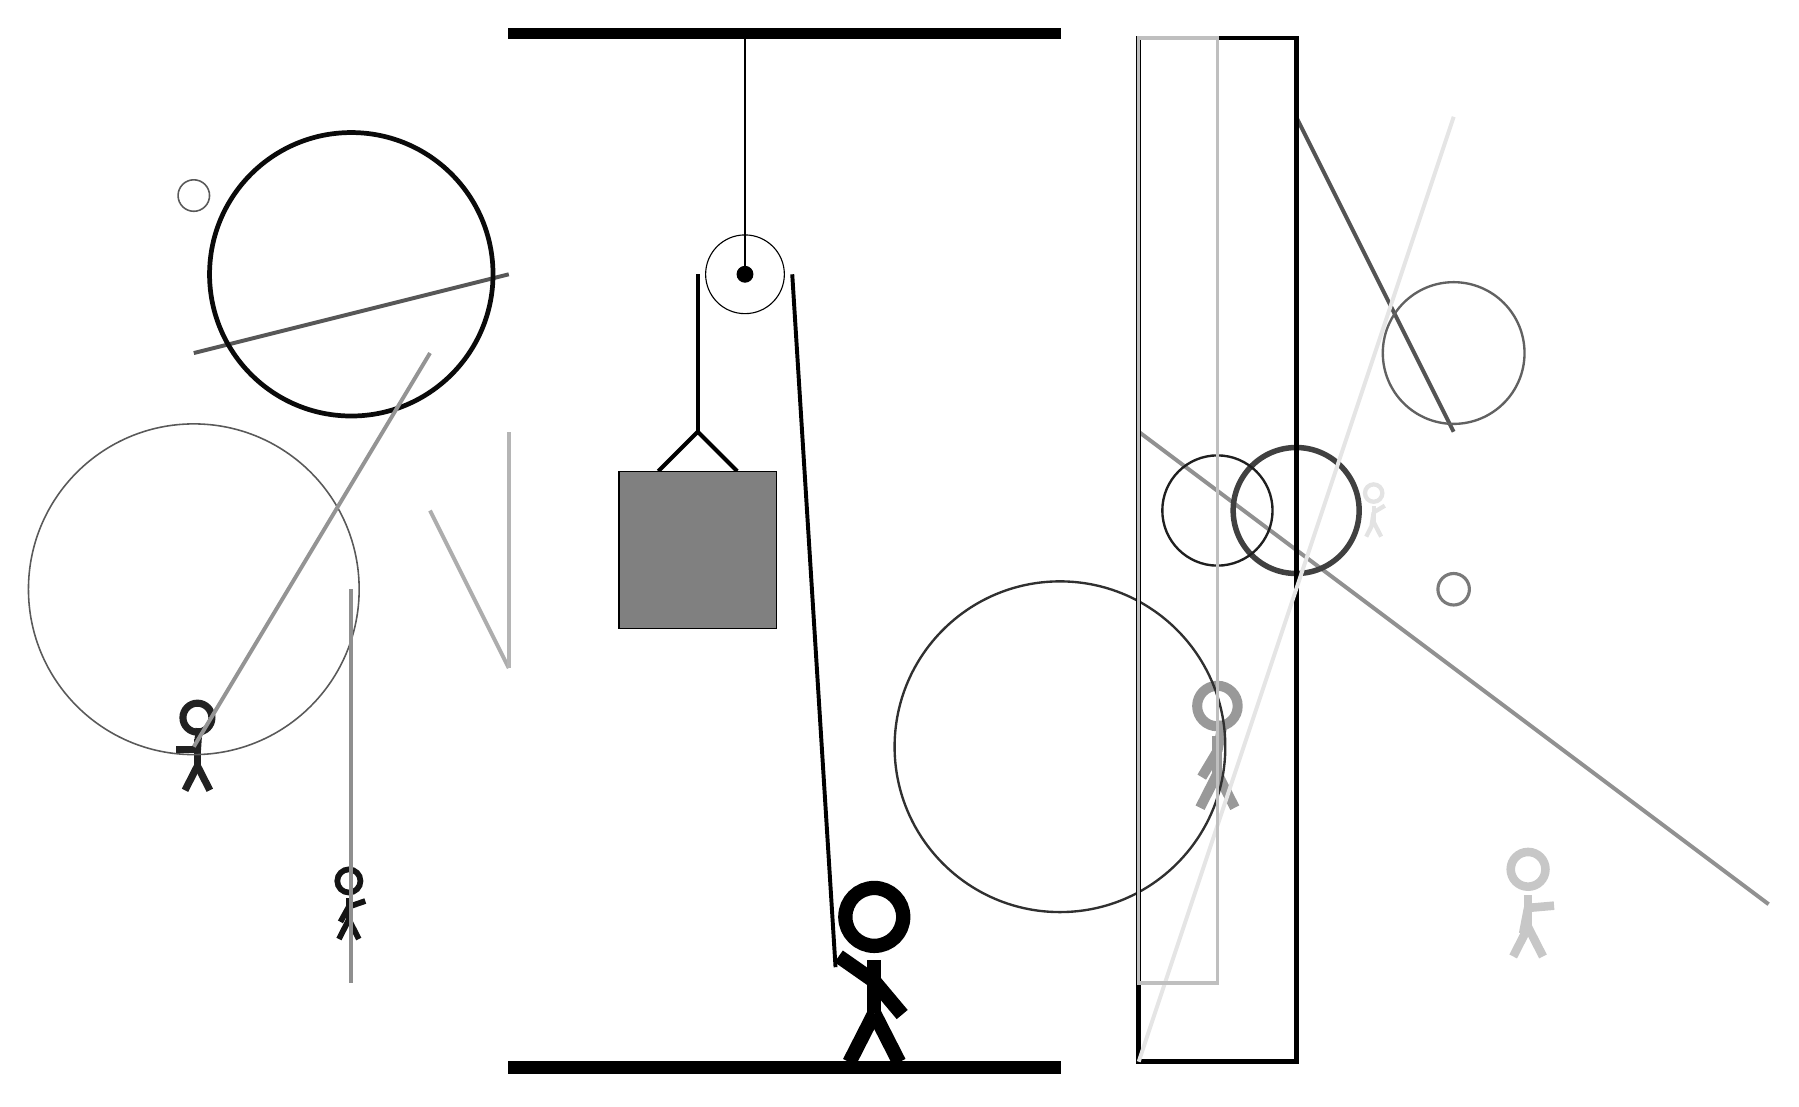
\begin{tikzpicture}
		%%%%% START %%%%%
		
		\draw[fill=black] (-2, 10) rectangle (5, 10.125);
		
		\draw (1, 7) circle (0.5);
		\draw[fill=black] (1, 7) circle (0.1);
		\draw (1, 10) -- (1, 7);
		
		\draw[line width=0.5mm, color=black!32](-3, 4) -- (-2, 2);
		
		\node[line width=0.3mm, color=black!11] at (9, 4) {\Strichmaxerl[3][81][31]};
		\draw[line width=0.5mm, color=black!43](6, 5) -- (14, -1);
		\draw [line width=0.7mm, color=black!75](8, 4) circle (0.8);
		\draw[line width=0.5mm, color=black!67](8, 9) -- (10, 5);
		\draw [line width=0.4mm, color=black!52](10, 3) circle (0.2);
		\draw[line width=0.5mm, color=black!66](-6, 6) -- (-2, 7);
		\node[line width=0.6mm, color=black!92] at (-4, -1) {\Strichmaxerl[4][61][19]};
		\node[line width=0.4mm, color=black!40] at (7, 1) {\Strichmaxerl[7][59][79]};
		\draw [line width=0.3mm, color=black!88](7, 4) circle (0.7);
		\draw[line width=0.5mm, color=black!29](-2, 2) -- (-2, 5);
		\node[line width=0.3mm, color=black!87] at (-6, 1) {\Strichmaxerl[5][0][86]};
		\draw [line width=0.2mm, color=black!65](-6, 3) circle (2.1);
		
		\draw [line width=0.3mm, color=black!81](5, 1) circle (2.1);
		\draw [line width=0.6mm, color=black!96](-4, 7) circle (1.8);
		\draw [line width=0.3mm, color=black!62](10, 6) circle (0.9);
		
		\draw[line width=0.6mm, color=black!100] (6, -3) rectangle (8, 10);
		\draw [line width=0.2mm, color=black!65](-6, 8) circle (0.2);
		\node[line width=0.3mm, color=black!22] at (11, -1) {\Strichmaxerl[6][79][5]};
		\draw[line width=0.5mm, color=black!42](-3, 6) -- (-6, 1);
		\draw[line width=0.5mm, color=black!44](-4, -2) -- (-4, 3);
		\draw[line width=0.5mm, color=black!10](6, -3) -- (10, 9);
		
		\draw[line width=0.4mm, color=black!25] (7, 10) rectangle (6, -2);
		
		\draw[line width=0.5mm] (-0.1, 4.5) -- (0.4, 5.0) -- (0.9, 4.5);
		\draw[fill=black!50] (-0.6, 4.5) rectangle (1.4, 2.5);
		
		\draw[line width=0.5mm] (0.4, 7) -- (0.4, 5.0);
		\centerarc[line width=0.5mm](1, 7)(0:180:0.6);
		\draw[line width=0.5mm](1.6, 7) -- (2.15, -1.8);
		
		\node at (2.6, -1.9) {\Strichmaxerl[10][-35][-50]};
		
		\draw[fill=black] (-2, -3) rectangle (5, -3.15);
		
		%%%%% END %%%%%
	\end{tikzpicture}
\end{document}